\documentclass[a4paper,12pt]{scrartcl}
\usepackage[utf8]{inputenc}
\usepackage[ngerman]{babel}
\usepackage[T1]{fontenc}
\usepackage{amsmath}
\usepackage{stmaryrd}
\usepackage{wasysym}
\usepackage{lmodern}
\usepackage{graphicx}
\usepackage{paralist}
\usepackage{upgreek}
\usepackage{subfigure}
\usepackage{tipa}
\usepackage{amssymb}
\usepackage{gensymb}
\usepackage{dsfont}
\usepackage{mathtools}
\usepackage{ stmaryrd }
\usepackage{fancyhdr}

%\title{Abgabe 1}
%\author{Rafael Heid, Julian Deinert, Sabrina Buczko Gruppe\\ 6 und 7}
%\date{Abgabe am 24.10.16}

\gdef\blatt{FGI-2 Aufgabenblatt 03}

\title{\blatt}
\date{Gruppe 06}
\author{Sabrina Buczko 6663234, Julian Deinert 6535880, Rafael Heid 6704828}


\pagestyle{fancy}
\fancyhf{}
\fancyhead[L]{\blatt}
\fancyhead[R]{Buczko, Deinert, Heid}
\fancyfoot[C]{\thepage}

\begin{document}
\maketitle
\newpage
\setcounter{section}{2}
\section{}
\setcounter{subsection}{2}
\subsection{}
\subsubsection{}
$L(A_1)=\{\lambda\} oder (\{a,c\}\cdot\{b\})^*$\\
$L(A_2)=\{a,c\}\cdot\{b\}^* \cdot \{a,c\}\cdot \{a\}^* \cdot(\{b\}\cdot \{a,c\}\cdot\{b\}^* \cdot \{a,c\}\cdot \{a\}^*)^*$\\
$L^\omega (A_1)=(\{a,c\}\cdot\{b\})^\omega$\\
$L^\omega (A_2)=(\{a,c\}\cdot\{b\}^* \cdot \{a,c\}\cdot \{a\}^* \cdot\{b\})^\omega$

\subsubsection{}
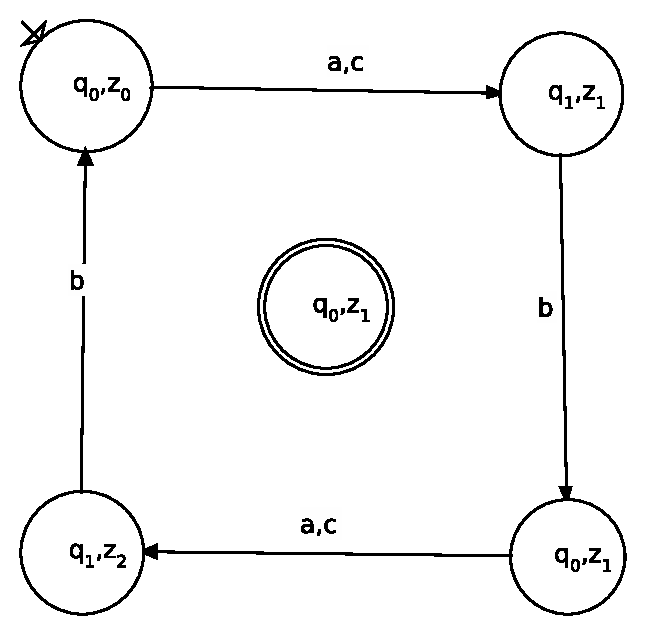
\includegraphics[scale=0.7]{334.pdf}

\subsubsection{}
$L(A_{3}) = \emptyset$\\
$L^\omega(A_{3}) = \emptyset$\\

\subsection{}
\subsubsection{}
Für $TS_1 \leftrightarroweq TS_2$\\
$\mathcal{B} = \{(z_0,p_0),(z_2,p_8),(z_1,p_1),(z_2,p_2),(z_0,p_3),(z_1,p_4),(z_2,p_5),(z_0,p_6),(Z2,P4),(z_1,p_7)\}$\\
Für $TS_1 \leftrightarroweq TS_3$\\
$\mathcal{B} = \{(z_0,q_0),(z_2,q_1),(z_1,q_2),(z_2,q_3),(z_0,q_4),(z_2,q_5),(z_1,q_6),(z_2,q_7),(z_0,q_8),(z_2,q_9)....\}$\\
Für $TS_2 \leftrightarroweq TS_3$\\
$\mathcal{B} = \{(p_0,q_0),(p_8,q_1),(p_1,q_2),(p_2,q_3),(p_0,q_4),(p_8,q_5),(P3,Q4),(P2,Q5),(p_4,q_6),()\}$\\


\end{document}
